 
\chapter{An Econometric Perspective of the Instrumental Variable}
 \label{chapter::iv-econometric}
 
 
Chapters \ref{chapter::iv-experiment} and \ref{chapter::iv-inequalities} discuss the IV method from the experimental perspective. Figure \ref{fig::causal-diagram-IV} illustrates the intuition behind the discussion. 
 
 
\begin{figure}[h]
\centering 
$
\xymatrix{
 && & U  \ar[dl] \ar[dr] &\\
Z \ar[rr] &&D \ar[rr]&&Y
}
$
\caption{Causal diagram for IV}\label{fig::causal-diagram-IV}
\end{figure} 
 
 
 
In an encouragement design with noncompliance, $Z$ is randomized, so it is independent of the confounder $U$ between the treatment received $D$ and the outcome $Y$.  Importantly, the treatment assignment $Z$ does not have any direct effect on the outcome $Y$. It acts as an IV for the treatment received $D$ in the sense that it affects the outcome $Y$ only through the treatment received $D$. This IV is generated by the experimenter. 


In many applications, randomization is infeasible. Then how can we draw causal inference in the presence of unmeasured confounding between the treatment $D$ and outcome $Y$? A clever idea from econometrics is to find {\it natural experiments} to mimic the setting of encouragement designs. To identify the causal effect of $D$ on $Y$ with unmeasured confounding, we can find another variable $Z$ that satisfies the assumptions of the diagram in Figure \ref{fig::causal-diagram-IV}.  The variable $Z$ must satisfy the following conditions:
\begin{enumerate}
\item
it should be close to being randomized so that it is independent of the unmeasured confounding $U$;
\item
it should change the distribution of $D$;
\item
it should affect the outcome $Y$ only indirectly through $D$ but not directly.
\end{enumerate}
If all these conditions hold, then $Z$ is a valid IV for estimating the effect of $D$ on $Y$. 



This chapter will provide the traditional econometrics perspective on IV. It is based on linear regression. \citet{imbens1994identification} and \citet{angrist1996identification} made a fundamental contribution by clarifying the connection between this perspective and the experimental perspective in Chapters \ref{chapter::iv-experiment} and \ref{chapter::iv-inequalities}. I will start with examples and then give more algebraic details. 



\section{Examples of studies with IVs}
 
 
 
Finding IV for causal inference is more an art than a science. The algebraic details in later sections are not the most complicated ones in statistics. However, it is fundamentally challenging to find IVs in empirical research. Below are some famous examples.  


\begin{example} 
In an encouragement design, $Z$ is the randomly assigned treatment, $D$ is the final treatment received, and $Y$ is the outcome. The IV assumptions encoded by Figure \ref{fig::causal-diagram-IV} are plausible in double-blind RCTs as discussed in Chapter \ref{chapter::iv-experiment}. This is the ideal case for IV. 
\end{example}


 
 
 \begin{example}
 \citet{hearst1986delayed}   reported that men with low lottery numbers in the Vietnam Era draft lottery had higher mortality rates afterward.  They attributed this to the negative effect of military service.
 \citet{angrist1990lifetime} further reported that men with low lottery numbers in the Vietnam Era draft lottery had lower subsequent earnings. He attributed this to the negative effect of military service. 
 These explanations are plausible because the lottery numbers were randomly generated, men with low lottery numbers were more likely to have military service, and the lottery numbers were unlikely to affect the subsequent mortality or earnings. That is, Figure \ref{fig::causal-diagram-IV} is plausible. 
\citet{angrist1996identification} reanalyzed the data using the IV framework. Here, the lottery number is the IV, military service is the treatment, and mortality or earnings is the outcome. 
\end{example}




\begin{example}
\citet{angrist1991does} studied the return of schooling in years on earnings, using the quarter of birth as an IV. This IV is plausible because of the pseudo-randomization of the quarter of birth.  It affected the years of schooling because (1) most states in the U.S. required the students to enter school in the calendar year in which they turned six, and (2) compulsory schooling laws typically required students to remain in school before their sixteenth birthday. More importantly, it is plausible that the quarter of birth did not affect earnings directly. 
\end{example}


\begin{example}
\citet{angrist1998children} studied the effect of family size on mothers' employment and work, using the sibling sex composition as an IV. This IV is plausible because of the pseudo-randomization of the sibling sex composition. Moreover, parents in the U.S. with two children of the same sex are more likely to have a third child than those parents with two children of different sex. It is also plausible that the sibling sex composition does not affect the mother's employment and work directly. 
\end{example}


\begin{example}\label{example::Card1993}
\citet{card1993using} studied the effect of schooling on wages, using the geographic variation in college proximity as an IV. In particular, $Z$ contains dummy variables for whether a subject grew up near a two-year college or a four-year college. Although this study is classic, it might be a poor example for IV because parents' choices of where to live might not be random, and moreover, where a subject grew up might matter for the subsequent wage. 
\end{example}



\begin{example}
\citet{voight2012plasma} studied the causal effect of plasma high-density lipoprotein (HDL) cholesterol on the risk of heart attack based on {\it Mendelian randomization}. They used some single-nucleotide polymorphisms (SNPs) as genetic IV for HDL, which are random with respect to the unmeasured confounders between HDL and heart attack by Mendel's second law, and affect heart attack only through HDL. 
I will give more details of Mendelian randomization in Chapter \ref{chapter::iv-mr}. 
\end{example}



\section{Brief Review of the Ordinary Least Squares}



Before discussing the econometric view of IV, I will first review the OLS (see Chapter \ref{appendix::basic-linear-regression}). This is a standard topic in statistics. However, it has different mathematical formulations, and the choice of formulation matters for the interpretation. 

The first view is based on projection.  Given a random variable $Y$ and a random variable or vector $D$  with finite second moments, define the population OLS coefficient as
\begin{eqnarray*}
\beta  &=& \arg\min_b E(Y - D  \tran b  )^2 \\
&=& E(DD\tran)^{-1} E(DY),
\end{eqnarray*}
and then define the population residual as $\varepsilon = Y -  D  \tran \beta $. By definition, $Y$ decomposes into 
\begin{eqnarray}\label{eq::olsdecomposition}
Y = D  \tran \beta  + \varepsilon,
\end{eqnarray}
which must satisfy 
$$
E(  D \varepsilon) = 0.
$$ 
Based on  $(D_i,Y_i)_{i=1}^n \iidsim (D, Y)$, the OLS estimator of $\beta$ is the  moment estimator
$$
\hat{\beta} = \left(  \sumn D_i D_i\tran \right)^{-1}   \sumn D_i Y_i  . 
$$
Because
\begin{eqnarray*}
\hat{\beta}  &=& \left(  \sumn D_i D_i\tran \right)^{-1}  \sumn D_i ( D_i\tran \beta + \varepsilon_i   )  \\
&=& \beta + \left(  \sumn D_i D_i\tran \right)^{-1} \sumn D_i  \varepsilon_i   ,
\end{eqnarray*}
we can show that $\hat{\beta}$ is consistent for $\beta$ by the law of large numbers and the fact $E(\varepsilon D) = 0.$ 
The classic EHW robust variance estimator for $\cov(\hat\beta)$ is
$$
\hat{V}_\textsc{ehw} = \left(  \sumn D_i D_i\tran \right)^{-1}
\left(  \sumn \hat{\varepsilon}_i^2 D_i D_i\tran \right)
\left(  \sumn D_i D_i\tran \right)^{-1}
$$
where $\hat{\varepsilon}_i  = Y_i - D_i\tran \hat{\beta}$ is the residual. 




The second view is to treat
\begin{eqnarray}\label{eq::ols-true-model}
Y = D  \tran \beta  + \varepsilon,
\end{eqnarray}
as a true model for the data-generating process. 
That is, given the random variables $(D, \varepsilon)$, we generate $Y$ based on the linear equation \eqref{eq::ols-true-model}.
Importantly, in the data-generating process, $\varepsilon$ and $D$ may be correlated with $E( D \varepsilon) \neq  0$.  Figure \ref{fig::endogenous-regressor} gives such an example. This is the fundamental difference compared with the first view where $E(\varepsilon D) = 0$ holds by the definition of the population OLS. 
Consequently, the OLS estimator can be inconsistent:
$$
\hat{\beta} \rightarrow \beta + E(DD\tran)^{-1} E(D\varepsilon) \neq \beta 
$$
in probability, as the sample size $n$ approaches infinity. 


I end this section with definitions of {\it endogenous} and {\it exogenous} regressors based on \eqref{eq::ols-true-model}, although their definitions are not unique in econometrics. 



\begin{definition}
\label{def::endogenous-exogenous}
When $E(\varepsilon D) \neq  0$, the regressor $D$ is called {\it endogenous}; when $E(\varepsilon D) =  0$, the regressor $D$ is called {\it exogenous}. 
\end{definition}

The terminology in Definition \ref{def::endogenous-exogenous} is standard in econometrics. 
When $E(\varepsilon D) \neq  0$, we also say that we have {\it endogeneity}; when $E(\varepsilon D) =  0$, we also say that we have {\it exogeneity}.

In the first view of OLS, the notions of endogeneity and exogeneity do not play any roles because $E(\varepsilon D) =  0$ by definition.  Statisticians holding the first view usually find the notions of endogeneity and exogeneity strange, and consequently, find the idea of IV unnatural. To understand the econometric view of IV, we must switch to the second view of OLS. 




 

\begin{figure}[h]
\centering
\begin{subfigure}[]{0.4\textwidth}
                \centering
$
\xymatrix{
& U \ar[dl] \ar[dr]& \\
D \ar[dr] & & \varepsilon \ar[dl] \\
&Y&
}
$                \caption{$E(D\varepsilon) \neq 0$}
        \end{subfigure}%
        
        \begin{subfigure}[]{0.4\textwidth}
                \centering
$
\xymatrix{
&\varepsilon  \ar[dl] \ar[dr] &\\
D \ar[rr]&&Y
}
$
                \caption{marginalized over $\varepsilon$}
        \end{subfigure}%
        
\caption{ Different representations of the endogenous regressor $D$. In the upper panel, $U$ represents unmeasured common causes of $D$ and $\varepsilon$.}\label{fig::endogenous-regressor}
\end{figure}



\section{Linear Instrumental Variable Model}
\label{sec::linear-iv-model}



When $D$ is endogenous, the OLS estimator is inconsistent. We must use additional information to construct a consistent estimator for $\beta$. 
I will focus on the following linear IV model:


\begin{definition}
[linear IV model]\label{def::linear-iv-model}
We have 
$$
Y = D  \tran \beta  + \varepsilon ,
$$
with
\begin{eqnarray}\label{eq::iv-moment-condition}
E(\varepsilon Z) = 0 . 
\end{eqnarray}
\end{definition}


The linear IV model in Definition \ref{def::linear-iv-model} can be illustrated by the following causal graph: 
%\begin{figure}[h]
%\centering 
$$
\xymatrix{
&&&\varepsilon  \ar[dl] \ar[dr] &\\
Z\ar[rr]&&D \ar[rr]&&Y
}
$$
%\caption{Instrumental variable}
%\end{figure}

The above linear IV model allows that $E(\varepsilon D) \neq 0$ but requires an alternative moment condition \eqref{eq::iv-moment-condition}. With $E(\varepsilon) = 0$ by incorporating the intercept, the new condition states that $Z$ is uncorrelated with the error term $\varepsilon$. But any randomly generated noise is uncorrelated with $\varepsilon$, so an additional condition must hold to ensure that $Z$ is useful for estimating $\beta$. Intuitively, the additional condition requires that $Z$ is correlated to $D$, with more technical details stated below.  
 

The mathematical requirement \eqref{eq::iv-moment-condition} seems simple. However, it is a key challenge in empirical research to find such a variable $Z$ that satisfies \eqref{eq::iv-moment-condition}. Since the condition \eqref{eq::iv-moment-condition} involves the unobservable $\varepsilon$, it is generally untestable. 
 


\section{The Just-Identified Case}
\label{sec::iv-just-identify}

We first consider the case in which $Z$ and $D$ have the same dimension and $E(ZD\tran)$ has full rank. The condition $E(\varepsilon Z) = 0$ implies that
$$
E\{  Z (Y -  D \tran \beta) \} = 0 .
$$
Solve the linear equations to obtain
$$
E(  ZY)  = E(ZD\tran) \beta  \\
 \Longrightarrow 
\beta = E(ZD\tran) ^{-1} E(  ZY)  
$$
if $E(ZD\tran)$ is not degenerate. 
The OLS is a special case if $E(\varepsilon D) = 0$, i.e., $D$ acts as an IV for itself. The resulting moment estimator is
\begin{eqnarray}\label{eq::iv-estimator}
\hat{\beta}_\textsc{iv} = \left(  \sumn Z_i D_i\tran \right)^{-1}  \sumn Z_iY_i.
\end{eqnarray}

It can be insightful to work out the details for the case with a  scalar $D$ and $Z$. See Example \ref{eg::scalar-iv} below.

\begin{example}\label{eg::scalar-iv}
In the simple case with an intercept and scalar $D$ and $Z$, we have  the model
$$
\left\{ \begin{array}{l}
Y = \alpha +  \beta  D + \varepsilon ,\\
E(\varepsilon) = 0, \quad \cov(\varepsilon, Z) = 0,
\end{array}
\right.
$$
Under this model, we have 
$$
\cov( Z, Y ) = \beta \cov(Z, D) 
$$
which implies
$$
 \beta = \frac{ \cov( Z, Y )   }{ \cov(Z, D) }.
$$
Standardize the numerator and denominator by $\var(Z)$ to obtain 
$$
\beta =  \frac{ \cov( Z, Y ) / \var(Z)  }{ \cov(Z, D) / \var(Z) },
$$
which equals the ratio between the coefficients of $Z$ in the OLS fits of $Y$ and $D$ on $Z$. 
If $Z$ is binary, these coefficients are differences in means (see Problem \ref{problem::pols-binary}), and $\beta$ reduces to
$$
\beta = \frac{ E(Y\mid Z=1) - E(Y\mid Z=0)  }{ E(D\mid Z=1) - E(D\mid Z=0) } .
$$
This is identical to the identification formula in Theorem \ref{thm::CACE-identification}. That is, with a binary IV $Z$ and a binary treatment $D$, the IV estimator recovers the CACE under the potential outcomes framework. This is a key result in  \citet{imbens1994identification} and \citet{angrist1996identification}.  
\end{example}



 

\section{The Over-Identified Case}
\label{sec::sec::iv-over-identify}

The discussion in Section \ref{sec::iv-just-identify} focuses on the {\it just-identified} case.  When $Z$ has a lower dimension than $D$ and $E(ZD\tran)$ does not have full column rank, the equation $E(  ZY)  = E(ZD\tran) \beta$ has infinitely many solutions. This is the {\it under-identified} case in which the coefficient $\beta$ cannot be uniquely determined even with $Z$. It is a challenging case beyond the scope of this book. To ensure identifiability, we need at least as many IVs as the endogenous regressors. 

When $Z$ has a higher dimension than $D$ and $E(ZD\tran)$ has full column rank, we have many ways to determine $\beta$ from $E(  ZY)  = E(ZD\tran) \beta$. What is more,  the sample analog 
$$
n^{-1} \sumn Z_iY_i = n^{-1} \sumn Z_i D_i\tran \beta
$$
may not have any solution because the number of equations is larger than the number of unknown parameters. 


A computational trick for the over-identified case is the {\it two-stage least squares}  (TSLS) estimator \citep{theil1953estimation, basmann1957generalized}. It is a clever computational trick, which has two steps.

\begin{definition}
[Two-stage least squares]\label{def::2sls}
Define the TSLS estimator of the coefficient of $D$ with $Z$ being the IV as follows. 
\begin{enumerate}
\item
Run OLS of $D$ on $Z$, and obtain the fitted value $\hat{D}_i\ (i=1,\ldots, n)$. If $D_i$ is a vector, then we need to run component-wise OLS to obtain $\hat{D}_i$. Put the fitted vectors in a matrix $\hat{D}$ with rows $\hat{D}_i\tran $;
\item
Run OLS of $Y$ on $\hat{D}$, and obtain the coefficient $\hat{\beta}_\textsc{tsls}$.  
\end{enumerate}
\end{definition}
 

To see why TSLS works, we need more algebra. Write it more explicitly as
\begin{eqnarray} 
\hat{\beta}_\textsc{tsls} &=& \left(  \sumn \hat{D}_i\hat{D}_i\tran \right) ^{-1} 
\sumn \hat{D}_i Y_i  \label{eq::2sls-definition} \\
&=& \left(  \sumn \hat{D}_i\hat{D}_i\tran \right) ^{-1} 
\sumn \hat{D}_i (D_i \tran \beta + \varepsilon_i)  \nonumber  \\
&=& \left(  \sumn \hat{D}_i\hat{D}_i\tran \right) ^{-1} 
\sumn \hat{D}_i D_i \tran \beta + \left(  \sumn \hat{D}_i\hat{D}_i\tran \right) ^{-1} \sumn \hat{D}_i  \varepsilon_i .   \nonumber 
\end{eqnarray}  
The first stage OLS fit ensures $D_i  = \hat{D}_i + \check D_i$ with orthogonal fitted values and residuals, that is,
\begin{equation} \label{eq::ols-orthogonal}
\sumn \hat{D}_i  \check D_i\tran = 0
\end{equation}
is a zero square matrix with the same dimension as $D_i$. The orthogonality \eqref{eq::ols-orthogonal} implies 
$$
\sumn \hat{D}_i D_i \tran = \sumn \hat{D}_i\hat{D}_i\tran,
$$ 
which further implies that 
\begin{eqnarray}
\label{eq::2sls-ols}
\hat{\beta}_\textsc{tsls} = \beta + \left(  \sumn \hat{D}_i\hat{D}_i\tran \right) ^{-1} \sumn \hat{D}_i  \varepsilon_i.
\end{eqnarray}
The first stage OLS fit also ensures 
\begin{equation}
\label{eq::ols-donz}
\hat{D}_i = \hat{\Gamma}\tran  Z_i 
\end{equation}
which implies that
\begin{eqnarray}
\label{eq::2sls-consistency}
\hat{\beta}_\textsc{tsls} = \beta + \left\{  \hat{\Gamma}\tran  \left(  n^{-1}  \sumn Z_i Z_i\tran  \right) \hat{\Gamma}  \right\}  ^{-1}  
\hat{\Gamma}\tran  \left( n^{-1} \sumn Z_i  \varepsilon_i \right) . 
\end{eqnarray}
Based on \eqref{eq::2sls-consistency}, we can see the consistency of the TSLS estimator by the law of large numbers and the fact that the term $n^{-1} \sumn Z_i  \varepsilon_i $ has probability limit $E(Z\varepsilon) = 0$. We can also use \eqref{eq::2sls-consistency} to show that when $Z$ and $D$ have the same dimension,  $\hat{\beta}_\textsc{tsls} $ is numerically identical to $\hat{\beta}_\textsc{iv} $ defined in Section \ref{sec::iv-just-identify}, which is left  as Problem \ref{prob::algebra-tsls}. 




Based on \eqref{eq::2sls-ols}, we can obtain the standard error as follows. We first obtain the residual $\hat{\varepsilon}_i = Y_i - \hat{\beta}_\textsc{tsls}\tran D_i$, and then obtain the robust variance estimator as
$$
\hat{V}_\textsc{tsls} = \left( \sumn  \hat{D}_i \hat{D}_i\tran  \right)^{-1}
 \left( \sumn \hat{\varepsilon}_i ^2  \hat{D}_i \hat{D}_i\tran  \right)
\left( \sumn  \hat{D}_i \hat{D}_i\tran  \right)^{-1} . 
$$
Importantly, the $\hat{\varepsilon}_i$'s  are
not the residual from the second stage OLS $  Y_i - \hat{\beta}_\textsc{tsls}\tran \hat{D}_i $, so $\hat{V}_\textsc{tsls} $ differs from the robust variance estimator from the second stage OLS. 




\section{A Special Case: A Single IV for a Single Endogenous Treatment}


This section focuses on a simple case with a single IV and a single endogenous treatment. It has wide applications. 
Consider the following {\it structural equations}:
\begin{eqnarray}
\label{eq::strucrual-iv}
\left\{
\begin{array}{l}
Y_i = \beta_0 + \beta_1 D_i + \beta_2\tran X_i + \varepsilon_{i},\\
D_i = \gamma_0 + \gamma_1 Z_i + \gamma_2 \tran X_i + \varepsilon_{2i},
\end{array}
\right.
\end{eqnarray}
where $D_i$ is a scalar endogenous regressor representing the treatment variable of interest (i.e., $E(\varepsilon_{i} D_i) \neq 0$), $Z_i$ is a scalar IV for $D_i$ (i.e., $E(\varepsilon_{i} Z_i) = 0$), and $X_i$ contains other exogenous regressors (i.e., $E(\varepsilon_{i} X_i) = 0$). This is a special case with $D$ replaced by $(1, D, X)$ and $Z$ replaced by $(1, Z, X)$. 



\subsection{Two-stage least squares}

The TSLS estimator in Definition \ref{def::2sls} simplifies to the following form. 

\begin{definition}
[TSLS with a single endogenous regressor]\label{def::tsls-single}
Based on \eqref{eq::strucrual-iv}, the TSLS estimator has the following two steps.
\begin{enumerate}
\item
Run OLS of $D$ on $(1, Z,X)$, obtain the fitted values $\hat{D}_i\ (i=1,\ldots, n)$, and vectorize them as $\hat{D}$; 

\item 
Run OLS of $Y$ on $(1, \hat{D}, X)$, and obtain the coefficient $\hat{\beta}_\textsc{tsls}$, and in particular, $\hat{\beta}_{1,\textsc{tsls}}$, the coefficient of $\hat{D}$. 
\end{enumerate}
\end{definition}



\subsection{Indirect least squares}


The structural equation \eqref{eq::strucrual-iv} implies 
\begin{eqnarray*}
Y_i &=&\beta_0 + \beta_1 (\gamma_0 + \gamma_1 Z_i + \gamma_2 \tran X_i + \varepsilon_{2i}) + \beta_2\tran X_i + \varepsilon_{i} \\
&=& (\beta_0 + \beta_1\gamma_0 ) + \beta_1  \gamma_1 Z_i  + ( \beta_2 + \beta_1 \gamma_2 )\tran X_i  + ( \varepsilon_{i} + \beta_1 \varepsilon_{2i} ).
\end{eqnarray*}
Define $\Gamma_0 = \beta_0 + \beta_1\gamma_0, \Gamma_1  =  \beta_1  \gamma_1, \Gamma_2 = \beta_2 + \beta_1 \gamma_2$, and $\varepsilon_{1i} = \varepsilon_{i} + \beta_1 \varepsilon_{2i}$. We have the following equations
\begin{eqnarray}
\label{eq::reduced-iv}
\left\{
\begin{array}{l}
Y_i =\Gamma_0 + \Gamma_1 Z_i + \Gamma_2\tran X_i + \varepsilon_{1i},\\
D_i = \gamma_0 + \gamma_1 Z_i + \gamma_2 \tran X_i + \varepsilon_{2i},
\end{array}
\right.
\end{eqnarray}
which is called the {\it reduced form}, in contrast to the {\it structural form} in \eqref{eq::strucrual-iv}. The parameter of interest equals the ratio of two coefficients 
$$
\beta_1 = \Gamma_1 / \gamma_1.
$$ 
In the reduced form, the left-hand side are dependent variables $Y$ and $D$, and the right-hand side are the exogenous variable $Z$ and $X$ satisfying 
$$
E( Z \varepsilon_{1i} ) = E( Z \varepsilon_{2i} )  = 0, \quad 
E( X \varepsilon_{1i} ) = E( X \varepsilon_{2i} )  = 0.
$$ 
More importantly, OLS gives consistent estimators for the coefficients in the reduced form \eqref{eq::reduced-iv}. 


The reduced form \eqref{eq::reduced-iv} suggests that the ratio of two OLS coefficients $\hat{\Gamma}_1$ and $\hat{\gamma}_1$ is a reasonable estimator for $\beta_1$. This is called the {\it indirect least squares} (ILS) estimator:
$$
\hat{\beta}_{1,\textsc{ils}} =  \hat{\Gamma}_1 / \hat{\gamma}_1 .
$$
Interestingly, it is numerically identical to the TSLS estimator under \eqref{eq::strucrual-iv}.

\begin{theorem}
\label{thm::ils=2sls}
%Under \eqref{eq::strucrual-iv}, we have  
With a single endogenous treatment and a single IV in \eqref{eq::strucrual-iv}, we have 
$$
\hat{\beta}_{1,\textsc{ils}}   = \hat{\beta}_{1,\textsc{tsls}} . 
$$
\end{theorem}

Theorem \ref{thm::ils=2sls} is an algebraic fact. 
\citet[][Section A.3]{imbens2014instrumental} pointed it out without giving a proof. 
I relegate its proof to Problem \ref{para::tsls-ils}. The ratio formula makes it clear that the TSLS estimator has poor finite sample properties with a weak instrument variable, i.e., $\gamma_1 $ is close to zero. 



\subsection{Weak IV}

The following inferential procedure is simpler, more transparent, and more robust to weak IV. It is more computationally intensive though. 
The reduced form \eqref{eq::reduced-iv}  also implies that
\begin{eqnarray}
\label{eq::anderson-rubin-reg}
Y_i  - bD_i = (\Gamma_0 -b \gamma_0 ) +  (\Gamma_1  - b \gamma_1 ) Z_i
+ (\Gamma_2 - b \gamma_2  ) \tran X_i  + ( \varepsilon_{1i} -  b \varepsilon_{2i} )
\end{eqnarray}
for any $b$. 
At the true value $b = \beta_1$, the coefficient of $Z_i$ must be $0$. This simple fact suggests a confidence interval for $\beta_1$ by inverting tests for $H_0(b): \beta_1 = b$:
$$
\left\{ b:  | t_Z(b) | \leq z_{1-\alpha/2} \right\},
$$
where $t_Z(b) $ is the $t$-statistic for the coefficient of $Z$ based on the OLS fit of \eqref{eq::anderson-rubin-reg} with the EHW standard error, and $z_{1-\alpha/2}$ is the $1-\alpha/2$ upper quantile of the standard Normal random variable. 
This confidence interval is more robust than the Wald-type confidence interval based on the TSLS estimator. It is similar to the  FAR confidence set discussed in Chapter \ref{chapter::iv-experiment}. This procedure makes the TSLS estimator unnecessary. What is more, we only need to run the OLS fit of $Y$ based on the reduced form if the goal is to test $\beta_1 = 0$ under \eqref{eq::strucrual-iv}. 



\section{Application}\label{sec::tsls-application}

 

Revisit Example \ref{example::Card1993}. 
\citet{card1993using} used the National Longitudinal Survey of Young Men to estimate the causal effect of education on earnings. The data set contains 3010 men with ages between 14 and 24 in the year 1966, and \citet{card1993using} leveraged the geographic variation in college proximity as an IV for education. Here, $Z$ is the indicator of growing up near a four-year college, $D$ measures the years of education, and the outcome $Y$ is the log wage in the year 1976, ranging from 4.6 to 7.8. Additional covariates are race, age, and squared age, a categorical variable indicating living with both parents, single mom, or both parents, and variables summarizing the living areas in the past. 



\begin{lstlisting}
> library("car")
> ## Card Data
> card.data = read.csv("card1995.csv")
> Y = card.data[, "lwage"]
> D = card.data[, "educ"]
> Z = card.data[, "nearc4"]
> X = card.data[, c("exper", "expersq", "black", "south", 
+                   "smsa", "reg661", "reg662", "reg663", 
+                   "reg664", "reg665", "reg666", 
+                   "reg667", "reg668", "smsa66")]
> X = as.matrix(X)
\end{lstlisting}


Based on TSLS, we can obtain the following the point estimator and $95\%$ confidence interval. 
\begin{lstlisting}
> Dhat    = lm(D ~ Z + X)$fitted.values
> tslsreg = lm(Y ~ Dhat + X)
> tslsest = coef(tslsreg)[2]
> ## correct se by changing the residuals
> res.correct       = Y - cbind(1, D, X)%*%coef(tslsreg)
> tslsreg$residuals = as.vector(res.correct)
> tslsse = sqrt(hccm(tslsreg, type = "hc0")[2, 2])
> res = c(tslsest, tslsest - 1.96*tslsse, tslsest + 1.96*tslsse)
> names(res) = c("TSLS", "lower CI", "upper CI")
> round(res, 3)
    TSLS lower CI upper CI 
   0.132    0.026    0.237 
\end{lstlisting}


Using the strategy of the FAR confidence set, we can compute $p$-value as a function of $b$. 
\begin{lstlisting}
> BetaAR   = seq(-0.1, 0.4, 0.001)
> PvalueAR = sapply(BetaAR, function(b){
+   Y_b   = Y - b*D
+   ARreg = lm(Y_b ~ Z + X)
+   coefZ = coef(ARreg)[2]
+   seZ   = sqrt(hccm(ARreg)[2, 2])
+   Tstat = coefZ/seZ
+   (1 - pnorm(abs(Tstat)))*2
+ })
\end{lstlisting}
Figure \ref{fig::card-far-ci} shows the $p$-values for a sequence of tests for the coefficient of $D$ based on following \ri{R} code:
\begin{lstlisting}
> plot(PvalueAR ~ BetaAR, type = "l",
+      xlab = "coefficient of D",
+      ylab = "p-value",
+      main = "Fieller-Anderson-Rubin interval based on Card's data")
> point.est = BetaAR[which.max(PvalueAR)]
> abline(h = 0.05, lty = 2, col = "grey")
> abline(v = point.est, lty = 2, col = "grey")
> ARCI = range(BetaAR[PvalueAR >= 0.05])
> abline(v = ARCI[1], lty = 2, col = "grey")
> abline(v = ARCI[2], lty = 2, col = "grey")
\end{lstlisting}
We report the point estimate as the value of $b$ with the largest $p$-value as well as the confidence interval as the region of $b$ with $p$-values larger than 0.05. 
\begin{lstlisting}
> FARres = c(point.est, ARCI)
> names(FARres) = c("FAR est", "lower CI", "upper CI")
> round(FARres, 3)
 FAR est lower CI upper CI 
   0.132    0.028    0.282
\end{lstlisting}
Comparing the TSLS and FAR methods, the lower confidence limits are very close but the upper confidence limits are slightly different due to the possibly heavy right tail of the distribution of the TSLS estimator. Overall, the TSLS and FAR methods give similar results in this example because the IV is not weak. 
 


\begin{figure}
\centering 
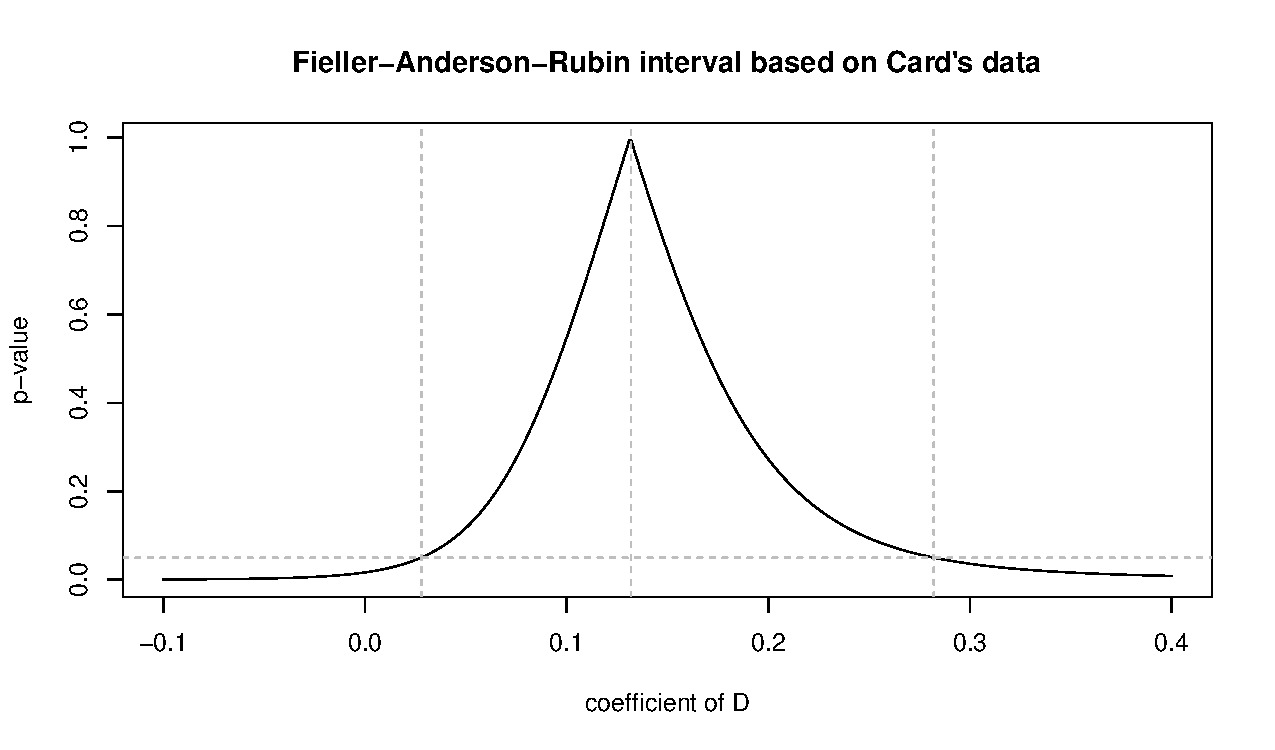
\includegraphics[width = \textwidth]{figures/FAR_Carddata.pdf}
\caption{Re-analysis of \citet{card1993using}'s data by inverting tests} \label{fig::card-far-ci} 
\end{figure}

 
 
 
\section{Homework}

\paragraph{More algebra for TSLS in Section \ref{sec::sec::iv-over-identify}}\label{prob::algebra-tsls}

\begin{enumerate}
\item 
Show that the $\hat \Gamma$ in \eqref{eq::ols-donz} equals
$$
\hat{\Gamma} = \left(  \sumn Z_i Z_i\tran  \right)^{-1} \sumn Z_i D_i\tran .
$$

\item
Show $\hat{\beta}_\textsc{tsls} $ defined in \eqref{eq::2sls-definition} reduces to $ \hat{\beta}_\textsc{iv}$ defined in \eqref{eq::iv-estimator} if $Z$ and $D$ have the same dimension and
$$
n^{-1} \sumn Z_i Z_i\tran, \quad n^{-1} \sumn Z_i D_i\tran
$$
are both invertible. 
\end{enumerate}

\paragraph{Equivalence between TSLS and ILS}\label{para::tsls-ils}
Prove Theorem \ref{thm::ils=2sls}. 


Remark: Use the FWL theorem in Chapter \ref{appendix::basic-linear-regression}. 



\paragraph{Control function in the linear instrumental variable model}\label{para::control-function-iv}

Definition \ref{def::cf} below parallels Definition \ref{def::2sls} above.

\begin{definition}
[control function]\label{def::cf}
Define the control function estimator $\hat{\beta}_\textsc{cf}$ as follows.
\begin{enumerate}
\item
Run OLS of $D$ on $Z$, and obtain the residuals $\check D_i\ (i=1,\ldots, n)$. If $D_i$ is a vector, then we need to run component-wise OLS to obtain $\check D_i$. Put the residual vectors in a matrix $\check{D}$ with rows $\check{D}_i\tran $;
\item
Run OLS of $Y$ on $D$ and $\check{D}$, and obtain the coefficient of $D$, $\hat{\beta}_\textsc{cf}$.  
\end{enumerate}
\end{definition}
 
 Show that $\hat{\beta}_\textsc{cf} = \hat{\beta}_\textsc{tsls}$.
 
 
 Remark:
To prove the result, you can use the results in Problems \ref{hw::ols-orthogonal} and \ref{hw::ols-transform-regressors}.  
  In Definition \ref{def::cf}, $\check{D}$ from Step 1 is called the control function for Step 2. 
 \citet{hausman1978specification} pointed out this result. \citet{wooldridge2015control} provided a more general discussion of the control function methods in more complex models. 
 
  


 

%\paragraph{Data analysis: \citet{card1993using}}
%
%\citet{card1993using} used the geographic variation in college proximity to estimate the return to schooling. The treatment is education and the outcome is log wage. The IV is the college proximity. 
%\texttt{card.csv} is a slightly modified version of the data from Card's homepage with detailed explanations of the variable names in \texttt{code\_bk.txt}.
%
%You can dichotomize the education variable and infer the LATE. How do you choose the threshold for the dichotomization? Are the results sensitive to your choice? Conduct an analysis with covariates. 
%
%Without dichotomizing the education variable, you can use the standard two-stage least squares estimator. Compare the results to the above analysis.
%
%What if the return of education is nonlinear? Do the data provide information for us to test the nonlinearity?
%


\paragraph{Data analysis: \citet{efron1991compliance}}

\citet{efron1991compliance} was one of the early studies dealing with noncompliance under the potential outcomes framework. The original randomized experiment, the Lipid Research Clinics Coronary Primary Prevention Trial (LRC-CPPT), was designed to evaluate the effect of the drug cholestyramine on cholesterol levels.
In the dataset \texttt{EF.csv}, the first column contains the binary indicators for treatment and control, the second column contains the proportions of the nominal cholestyramine dose actually taken, and the last three columns are cholesterol levels.
Note that the individuals did not know whether they were assigned to cholestyramine or to the placebo, but differences in adverse side effects could induce differences in compliance behavior by treatment status. All individuals were assigned the same nominal dose of the drug or placebo, for the same time period.
Column 3, $C_3$, was taken before communication about the benefits of a low-cholesterol diet, Column 4, $C_4,$ was taken after this suggestion, but before the random assignment to cholestyramine or placebo, and Column 5, $C_5$,  an average of post-randomization cholesterol readings, averaged over two-month readings for a period of time averaging 7.3 years for all the individuals in the study. \citet{efron1991compliance} used the change in cholesterol level as the final outcome of interest, defined as $C_5 - 0.25C_3 - 0.75C_4$. Their original paper contains more detailed descriptions. 
 

The data structure here is more complicated than the noncompliance problem discussed in Chapters \ref{chapter::iv-experiment} and \ref{chapter::iv-inequalities}. 
\citet{jin2008principal} re-analyzed the data based on the idea in Chapter \ref{chapter::principal-stratification} later. 
You can analyze the data based on your understanding of the problem, but you need to justify your choice of the method. There is no gold-standard solution for this problem. 




 \paragraph{Recommended reading}


\citet{imbens2014instrumental} gave an econometrician's perspective of IV. 

